\documentclass[a4paper,11pt]{article}

\usepackage[utf8]{inputenc}

\usepackage{graphicx}
\usepackage{caption}
\usepackage{subcaption}

\usepackage{pgfplots}
\pgfplotsset{compat=1.18} 

\usepackage{minted}
\usepackage{siunitx}

\begin{document}

\title{
    \textbf{Performance of Array Operations in C}
}
\author{Mo Wang}
\date{Spring 2026}

\maketitle

\section*{Introduction}

This report investigates the performance in terms of elapsed time of three array operations in C: random access of element, linear search of an element, and searching for duplicated elements in an array. As an introduction to algorithm and data structure, the purpose is to understand algorithms behavior such as time consumption in practice by measuring the elapsed time of each operation in arrays of different sizes. 

\section*{Benchmarking}

When it comes to measuring the elapsed time of an algorithm, there are some difficulties with measuring it. 

First of all, clock precision for timing an algorithm is limited. This is mainly due to the limited clock precision of \texttt{CLOCK\_MONOTONIC} in C from the POSIX \texttt{time.h} header, usually in orders of microseconds. Because of that, timing individual operations does not produce precise measurements and is thus unreliable, especially timing array access operation in orders of nanoseconds. To mitigate this issue, the same algorithm is executed over again multiple times, in my case 1024 times, while being batch timed. Afterwards, an average time can therefore be calculated from the batch time for 1024 loop for estimating each amortized elapsed time for one individual operation. Using this mitigation solution, an estimated and accurate time could be calculated.



Besides, the elapsed time differ in different computing systems and can also fluctuate when using the same computing system. Multiple factors can interfere with execution time, including hardware constraints, operating system time scheduler and background processes. To address this issue, same performance benchmark test is repeated a number of times, while an average elapsed time among the test result is calculated, in order to gain more accuracy.

In order to avoid compiler to optimize away performance benchmark code as dead code, the results of each operation are accumulated into a variable and read after the benchmark test loops. All arrays are allocated on the heap and initially filled with pseudo-random numbers in order to avoid cache locality and further optimizations that can obscure testing. For each benchmark, the array size is double as large as the previous one, in order to calculate a relevant scaling behavior and growth trend in a growing array size.

Finally, the reported numbers use an appropriate number of digits. The goal with the three benchmarks is not to claim unrealistic and arbitrary precision, but to illustrate clear performance trends as the input size increases.




This is what a report should look like; it is written using the
document class {\tt article} with {\tt a4paper} and {\tt 11pt}
options.

The name of the report should not be "My first report" and the name
should not be "My Name". I thought that would be obvious but each year
I have submitted reports were these templates have not been changed. 

What follows is a set of rules and hints on how to write you
reports. Follow these guidelines to make life easier and avoid failing
an assignment by including a screen shot. Do read these guidelines but
also look at the source code of this document. The code will hopefully
show you how to do things. It will also show what packages are
included to get things to work.

\section*{Random access}

The rows in regular article mode are short - because it makes it
easier to read. Do not set the column width or margins explicitly, let
LaTeX decide what it should look like.

Don't use any fancy packages that will turn your report into a
Christmas tree, keep it simple!.

\begin{table}[h]
\begin{center}
\begin{tabular}{l|c}
\textbf{Size of array} & \textbf{Time}\\
\hline
  1024   &  2.3 ns \\
  2048   &  2.4 ns \\
  4096   &  2.4 ns \\
  8192   &  2.3 ns \\
  16384  &  2.4 ns \\
  32768  &  2.3 ns \\
  65536  &  2.4 ns \\
  131072 &  4.8 ns \\
\end{tabular}
\caption{Union and friends, list of 50000 elements, runtime in microseconds}
\label{tab:table1}
\end{center}
\end{table}

A diagram here

\begin{figure}
  \centering
  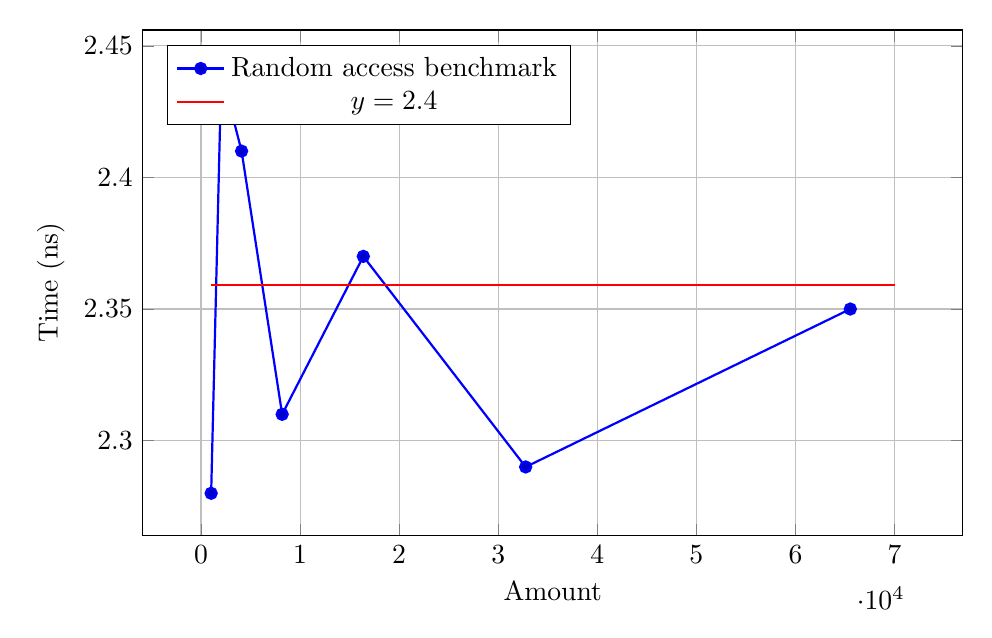
\begin{tikzpicture}
    \begin{axis}[
      xlabel={Amount},
      ylabel={Time (\si{\nano\second})},
      width=12cm, height=8cm,
      grid=major,
      legend pos=north west
    ]
      % Your benchmark data
      \addplot+[
        mark=*,
        thick,
        color=blue
      ] coordinates {
        (1024,   2.28)
        (2048,   2.44)
        (4096,   2.41)
        (8192,   2.31)
        (16384,  2.37)
        (32768,  2.29)
        (65536,  2.35)
      };
      \addlegendentry{Random access benchmark}

      \addplot[red, thick, domain=1000:70000] {2.359};
      \addlegendentry{$y = 2.4$}
      
    \end{axis}
  \end{tikzpicture}
  \caption{Random access benchmark with fitted line(s)}
  \label{fig:random-access}
\end{figure}


\section*{Array search benchmark}

The rows in regular article mode are short - because it makes it
easier to read. Do not set the column width or margins explicitly, let
LaTeX decide what it should look like.

Don't use any fancy packages that will turn your report into a
Christmas tree, keep it simple!.

\begin{table}[h]
\begin{center}
\begin{tabular}{l|c}
\textbf{Size of array} & \textbf{Time (approximate)}\\
\hline
  1024   &   1.7 µs   \\
  2048   &   3.3 µs   \\
  4096   &   6.4 µs   \\
  8192   &   13 µs    \\
  16384  &   26 µs    \\
  32768  &   51 µs    \\
  65536  &   100 µs   \\
  131072 &   200 µs   \\
\end{tabular}
\caption{Union and friends, list of 50000 elements, runtime in microseconds}
\label{tab:table1}
\end{center}
\end{table}

\begin{figure}
  \centering
  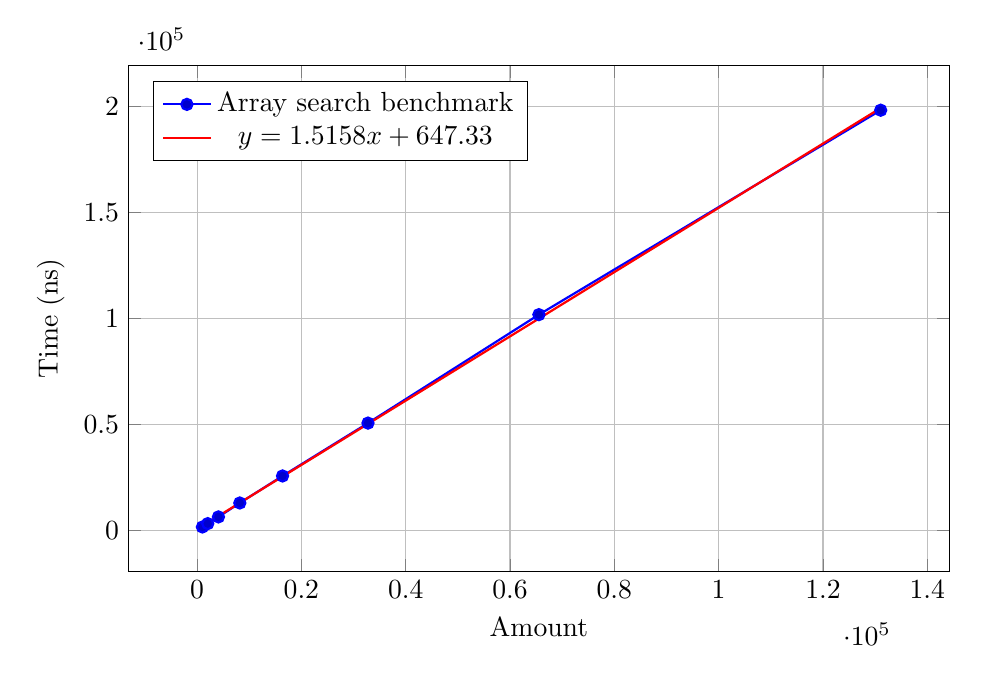
\begin{tikzpicture}
    \begin{axis}[
      xlabel={Amount},
      ylabel={Time (\si{\nano\second})},
      width=12cm, height=8cm,
      grid=major,
      legend pos=north west
    ]
      % Your benchmark data
      \addplot+[
        mark=*,
        thick,
        color=blue
      ] coordinates {
        (1024,   1679.10)
        (2048,   3268.07)
        (4096,   6436.80)
        (8192,   13010.31)
        (16384,  25751.70)
        (32768,  50693.34)
        (65536,  101850.42)
        (131072, 198295.30)
      };
      \addlegendentry{Array search benchmark}

      \addplot[red, thick, domain=0:131072] {1.5158*x + 647.33};
      \addlegendentry{$y = 1.5158x + 647.33$}
      
    \end{axis}
  \end{tikzpicture}
  \caption{Random access benchmark with fitted line(s)}
  \label{fig:random-access}
\end{figure}

\section*{Duplication}

\subsection*{sections}

Since this is a small report I can omit having numbered sections and
you do this by using section commands that end with a {\tt *} (for
example {\tt \textbackslash section* }). You can of course have
subsections etc. If you don't have numbers on the main sections,
don't add numbers to the subsections.

\begin{table}[h]
\begin{center}
\begin{tabular}{l|c}
\textbf{Size of array} & \textbf{Time (approximate)}\\
\hline
  1024   &  1.1 ms  \\  
  2048   &  3.7 ms  \\  
  4096   &  14 ms   \\ 
  8192   &  57 ms   \\ 
  16384  &  220 ms  \\  
  32768  &  890 ms  \\  
  65536  &  3.6 s   \\ 
  131072 &  14 s    \\
\end{tabular}
\caption{Union and friends, list of 50000 elements, runtime in microseconds}
\label{tab:table1}
\end{center}
\end{table}

\begin{figure}
  \centering
  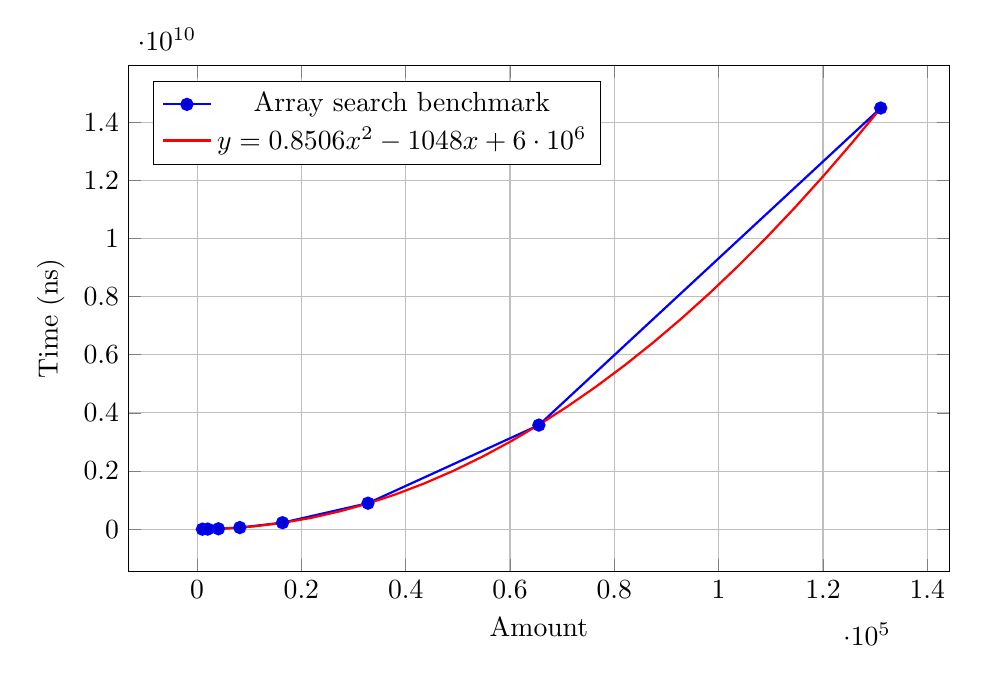
\begin{tikzpicture}
    \begin{axis}[
      xlabel={Amount},
      ylabel={Time (\si{\nano\second})},
      width=12cm, height=8cm,
      grid=major,
      legend pos=north west
    ]
      % Your benchmark data
      \addplot+[
        mark=*,
        thick,
        color=blue
      ] coordinates {
        (1024,   1065420.8)
        (2048,   3684608)
        (4096,   14206248.96)
        (8192,   56628264.96)
        (16384,  224418447.36)
        (32768,  894779381.76)
        (65536,  3580590469.12)
        (131072, 14484434739.2)
      };
      \addlegendentry{Array search benchmark}

      \addplot[red, thick, domain=0:131072] {0.8506*x^2 - 1048*x + 6e6};
      \addlegendentry{$y = 0.8506x^2 - 1048x + 6 \cdot 10^6$}
      
    \end{axis}
  \end{tikzpicture}
  \caption{Random access benchmark with fitted line(s)}
  \label{fig:random-access}
\end{figure}


\subsection*{inserting code}

Code snippets are included using the package {\tt minted}. If you
want to include a program statement in running text you can do this
using for example teletype-text: {\tt List.sort()}.

\begin{minted}{rust}
  for i in 0..10{
    sum += i;
  }
\end{minted}

The reports that you hand in should be four pages long - but not four
pages of code! Use code snippets where you want to describe how things
are done but don't include code just because you have written it. If
you include code you should comment the code in your report
i.e. explain why you include it.

\section*{numbers}

You will include some runtime measurements in your reports. You
should the think about the number of significant figures that you
use. Just because a benchmark took $1.2345678 s$ does not mean that
you should report it in this way. If you write this in your report
you're implicitly saying - if I do this again the number will be the
same. This could be true but I doubt that anything you do on a
computer can be determined with an 8 figure accuracy. The next time
you try it might very well take $1.2354678 s$. What you report is
maybe $1.235 s$ or $1.2 s$?

\subsection*{tables}

Numbers are often best presented in a table. You will have to do some
reading on how to format tables but the general structures is quite
easy. This is for example a table with some runtime figures.

\begin{table}[h]
\begin{center}
\begin{tabular}{l|c|c}
\textbf{prgm} & \textbf{runtime} & \textbf{ratio}\\
\hline
  dummy      &  115 &     1.0\\
  union      &  535 &     4.6\\
  tailr      &  420 &     3.6\\
\end{tabular}
\caption{Union and friends, list of 50000 elements, runtime in microseconds}
\label{tab:table1}
\end{center}
\end{table}

As you see in the table above, the runtime per se might not be
interesting. The interesting thing is how it relates to something
else. Look at the ratios above, it gives you the information that we
are looking for. So when you include numbers, ask your self why you
have these numbers in the report. What is the purpose, can you
describe it in a better way?


\section*{no f*ing screen shots}

I know that you are all very happy that things actually work and
eagerly want to show what things look like on you screen but please,
don't use {\em screen shots}. It looks ugly and it's impossible to mark or
copy the things that you want to show. It also, most often, show a lot
of irrelevant things so instead of using an image, copy the text and
format it so it's easy to read.

\begin{figure}
  \centering
  \includegraphics[scale=0.45]{screenshot.png}
  \label{fig:screenshot}
  \caption{This should never be used}
\end{figure}



\section*{graphs}


If you work with Gnuplot you should write the commands needed to
generate a diagram in a small script. Take a look in the file {\tt
  fib.p} and you will see how the diagram in Fig.\ref{fig:images} was
created from the data given in {\tt fib.dat} (the {\tt .png} file was
generated from {\tt fib.pdf} using the Linux {\tt convert}
program found in {\tt imagemagick}).

When you include graphs you should make sure that the images you
include are not raster images (gif, png etc) but a vector image that
scales when you zoom-in. In Fig.\ref{fig:images} you see the same
graph saved as a raster image (png) compared to a vector graphic
image. You might not see the difference but if you zoom-in you will
see that the vector image scales.

\begin{figure}[h]
  \centering
  \begin{subfigure}{.5\textwidth}
    \centering
    \includegraphics[scale=0.45]{fib.png}
    \caption{using raster graphics}
  \end{subfigure}%
  \begin{subfigure}{.5\textwidth}
    \centering
    \includegraphics[scale=0.45]{fib.pdf}
    \caption{using vector graphics.}
  \end{subfigure}
  \caption{Difference in image formats.}
  \label{fig:images}
\end{figure}

An alternative to including a graph produced by a separate program is
to describe the graph in \LaTeX. This can be done using the TikZ
library. This library is used to create all types of graphics and the
learning curve is quite steep. The benefit is that the \LaTeX document
becomes self contained and that you are in complete control over the result.

The data can either be written in the latex source file but better read
from a separate file. Reading from a separate file makes it easier to
combine the output from a benchmark with the report. If you construct
your benchmark to produce a file with the x and y values in columns
you can plot them using a simple {\tt \textbackslash addplot}
command. If you do changes to your program you simply run the
benchmark again and re-compile the \LaTeX file.

\begin{figure}
  \centering
  \begin{tikzpicture}
    \begin{axis}[
      xmin=12, xmax=28, ymin=0, ymax=3500,
      xlabel=n, ylabel={time in $\mu s$},
      width=8cm, height=6cm]
      \addlegendentry{runtime fib(n)};
      \addplot[] table {fib.dat};
    \end{axis}

  \end{tikzpicture}
  \caption{The same graph using TikZ}
  \label{fig:tikz}
\end{figure}

The graph in Fig.\ref{fig:tikz} is generated using Tikz and as you can
see, I know have the time in "$\mu s$" instead of in "us".


\section*{\LaTeX things}

Some \LaTeX errors that I frequently see that could easily be avoided
if you only know where they come from.

\section*{less than}

If you in your LaTeX code write "5 \textless\ 7" it will look like 5 <
7 and "9 \textgreater\ 7" will look like 9 > 7. Using the characters
\textless\ and \textgreater\ directly does not work ... so, how did I
do it?  I used the commands {\tt  \textbackslash textless} and {\tt
  \textbackslash textgreater} to generate the symbols \textless\ and
\textgreater.

You could also use {\tt \{\textbackslash tt 5 < 7\}} but then it
will use the teletype font and look like this: {\tt 5 < 7}.

Still another way is to write it using so called {\tt math mode}. This
is a mode used for writing mathematical formulas in a nice way. You
enclose your expression in {\tt \$} signs like this {\tt \$5 < 7\$}
and then it will look like this $5 < 7$.

If you have a larger mathematical expression you enclose it in double
\$ and the result is that it is written centered with some space
around it like this:  $$ 5 < (3 * 8 / 3 ) $$

\subsection{math mode}

There are several ways that you can write $n \log(n)$ in \LaTeX.

\begin{itemize}
\item {\tt \$n log(n)\$}  : which is interprated as $n xyz(n)$ i.e. $n \times l \times o \times g \times (n)$ and since we then omitt the multiplications it will be displayed as $n log(n)$

\item {\tt \$n \textbackslash times log(n)\$} : which is better since
  we then explicitly have one multiplication and it is displayed as
  $n \times log(n)$.

\item {\tt \$n \textbackslash log(n)\$} : which is how it should be
  done, its now displayed as $n \log(n)$.
\end{itemize}  



\subsection*{why strange font}

If you want to write {\em foo} in teletype font you write like this
\verb+{\tt foo}+. If you forget the closing \} then it will look like
this: {\tt foo. Now everything here after until the end of you report
  will look like this. }



\section*{make}

To automate a process of running benchmarks and compiling a report one
can add everything that needs to be done using a {\tt Makefile}. The
{\tt make} program will determine which files that needs to be
regenerated and re-do only the necessary steps. If you take a look at
the make-file that comes with this report you will see that a change
to the Fibonacci benchmark ({\tt fib.ex}) will trigger the file {\tt
  fib.dat} to be regenerated. This will in turn mean that he diagrams
are regenerated and in the end the \LaTeX report i recompiled.

Working with make-files that causes more than just the report to be
regenerated in one reason why it's more powerful to run \LaTeX on your
own machine rather than using {\em Overleaf}. It does require some
tinkering to get everything to work but once you have it up and running
the development cycle becomes much shorter.



\end{document}
